\documentclass{article}
\usepackage[utf8]{inputenc}
\usepackage[a4paper, left=25mm, right=25mm, top=20mm]{geometry}

\usepackage{graphicx}
\graphicspath{ {./images/} }
\usepackage{placeins}

\usepackage{biblatex}
\addbibresource{references-mendeley.bib}
\addbibresource{references.bib}

\usepackage{amsmath}
\usepackage{amssymb}
\usepackage{amsthm}
\usepackage{mathtools}

\usepackage[hidelinks]{hyperref}
\usepackage[nameinlink]{cleveref}

\newtheorem{proposition}{Proposition}[section]
\newtheorem{lemma}[proposition]{Lemma}

\title{Estimating the localized end-of-outbreak probability using Markov Chain Monte Carlo}
\author{Jack Buckingham}
\date{November 2021}

\begin{document}

\maketitle


\section{Introduction}
During an epidemic we tend to get many small, localised outbreaks. During such an outbreak, cases are monitored closely and measures may be put in place to minimise transmission. One problem is to assign a probability to there being any future cases given the cases observed so far. When this probability drops below a threshold determined by the decision maker, say 5\%, then the outbreak can be declared over, hence the name ``end-of-outbreak''.

This probability has been estimated previously for specific outbreaks in \cite{Linton2021}, \cite{Akhmetzhanov2021} and \cite{Nishiura2016}. The model used in these papers is a branching process with a random serial interval. However, as observed in \cite{Nishiura2016} where the method was first proposed, it does not properly condition on the observed data. In this report I estimate the exact probability conditional on the observed data, and compare this to the method from \cite{Linton2021}, \cite{Akhmetzhanov2021} and \cite{Nishiura2016}. For this, I will use the data from the hospital related outbreak of COVID-19 in Taiwan, studied in \cite{Akhmetzhanov2021}. Note however, that I will not attempt to account for a delay in reporting or under-ascertainment of cases as these papers do.

The need for a Markov Chain Monte Carlo (MCMC) method arises when we attempt to marginalise over the possible infection graphs consistent with the observed cases to date. This space is too large to compute the exact sum, and we appeal to Monte Carlo integration. We choose MCMC because we cannot sample directly from the posterior distribution over possible infection graphs, but do have access to a function proportional to this posterior. See \autoref{app:mcmc} for a brief review of the Metropolis-Hastings MCMC algorithm.

\section{Background}\label{sec:background}

In the branching process epidemic model, infections are organised into generations with each individual in the \((k+1)\)th generation either being infected by a unique individual in the \(k\)th generation, or being a case imported from outside the modelled population. Individuals in the model are also assigned an infection time by adding a random serial interval to the infection time of their parent infection. It is assumed that the number of direct infections, \(O_i\), caused by an individual \(i\) has a Negative-Binomial distribution, \(\mathcal{NB}(k, p)\), which is identical for all \(i\). Here \(p\) is defined in terms of the basic reproduction number, \(R_0\), and the shape parameter, \(k\). The full probability mass function is given by
\[p = \frac{R_0}{R_0 + k}, \qquad \mathbb{P}(O_i = e) = \frac{\Gamma(e + k)}{e! \Gamma(k)} p^e (1-p)^k \; \forall i.\]
The serial interval \(S_{ij}\) between infections \(i\) and \(j\) (where \(i\) infected \(j\)) is assumed to be a positive integer number of days and is also assumed to be identically distributed for all \(i, j\). The \(\{O_i\}\) and \(\{S_{ij}\}\) are assumed to be mutually independent.

Observations from this model come in the form of a sequence of values \(m_0, \dots, m_t\) counting the number of infections on each day from the start of the outbreak to the current time. We will write \(\mathcal{D}\) for the event of observing this data under the model. Number the observed cases chronologically from \(1\) to \(n\), breaking ties arbitrarily. We denote the corresponding infection times as \(t_1, \dots, t_n \leq t\), where \(t\) is our current observation horizon (i.e. the current time) and \(n\) is the number of observed infections.

We will need to set up some more notation in order to discuss this model. Given such a branching process and a corresponding set of observations up to time \(t\), let us write \(G_t\) for the directed graph determining who infected who within the observed cases. Write \(\tilde{G}_t\) for the full branching process to time \(t\), which comprises the infection graph \(G_t\), as well as the observed infection times \(t_1, \dots, t_n\).
% Write \(\tilde{G}\) to for the full branching process, without truncating at time \(t\).
Finally, in what follows we will need to condition on a particular set of `external' infections, imported from outside the population. Let \(\mathcal{E}\) be the event identifying a particular set of infection times for these external infections.

\section{Method}\label{sec:method}
Conditional on a particular infection graph, \(G_t\), explaining the observed infections, the probability that there will be no future infections can be shown to be (see \Cref{thm:conditional-eoo-prob})
\begin{equation}\label{eq:conditional-eoo-prob}
    \mathbb{P}(M(s) = 0 \;\forall s > t | G_t, \mathcal{D}) = \prod_{i=1}^n \left(1 - p q_i\right)^{e_i + k}
\end{equation}
where \(M(s)\) is the number of infections observed on day \(s\), \(q_i = \mathbb{P}(S > t-t_i)\) is the probability that a general infection seeded from an infection at time \(t_i\) will occur after our observation horizon \(t\), and \(e_i\) is the number of observed infections which are directly caused by individual \(i\) under \(G_t\). \autoref{eq:conditional-eoo-prob} gives the probability which should be used when we have exact knowledge of the infection graph, such as in a contact tracing study.

When we do not know the infection graph, we must condition and marginalise over a distribution of infection graphs which might explain our observed infections
\begin{equation}\label{eq:marginalise-graph}
    \mathbb{P}(M(s) = 0 \;\forall s > t | \mathcal{D}) = \sum_{G_t} \mathbb{P}(M(s) = 0 \;\forall s > t | G_t, \mathcal{D}) \mathbb{P}(G_t | \mathcal{D}).
\end{equation}
This is a sum over \((n-1)!\) terms, which means it is impractical to compute naïvely for even a modestly sized outbreak. For example, in the dataset I examine in this report, there are 21 observed cases giving over \(10^{19}\) terms in the sum. Therefore, we must turn to a numerical method such as MCMC.

We can compute a quantity proportional to the posterior \(\mathbb{P}(G_t | \mathcal{D})\) using Bayes rule (see \Cref{thm:conditional-graph-prob})
\begin{equation}
    \mathbb{P}(G_t | \mathcal{D}) \propto \mathbb{P}(\mathcal{E} | \mathcal{D}) \prod_{i=1}^n \frac{1}{(1-pq_i)^{e_i + k}} \underbrace{\frac{\Gamma(e_i + k)}{e_i! \Gamma(k)} p^{e_i} (1-p)^k}_{\mathcal{NB}(k, p) \;\text{p.m.f.}} \prod_{j:\, i \to j} \mathbb{P}(S = s_{ij}).
\end{equation}
Here \(S\) is a generic serial interval and \(s_{ij}\) is the serial interval observed between infections \(i\) and \(j\), and the final product is over individuals \(j\) who were directly infected by individual \(i\). The probability \(\mathbb{P}(\mathcal{E}|\mathcal{D})\) is the probability of the imported cases implicitly specified in \(G_t\) being correct, and should be specified by an expert. For the purpose of this report I will assume that this is an indicator function for a specific set of external infections. That is, after looking at the data, we classify each infection as either imported or not. Observing that \autoref{eq:marginalise-graph} is of the form \(\mathbb{E}_{G_t | \mathcal{D}}[g(G_t)]\), we can apply MCMC to estimate the probability of future infections.

We use the following proposal method, which gives an asymmetric proposal distribution:
\begin{itemize}
    \item \emph{Select an individual uniformly at random whose parent we will change.} This individual should be selected from individuals whose parent can be changed (i.e. those with at least one other possible parent with nonzero probability for the corresponding serial interval). Further, since we are considering a scenario with a fixed set of external cases, we do not change which infections were imported.
    \item \emph{Select a new parent for this individual} from the other possible parents, proportional to the probability of observing a serial interval of that size.
\end{itemize}
The reason for using the serial interval distribution to weight the proposal distribution is to encourage better mixing in the Markov Chain. Empirically I found that a chain with a uniform distribution for the new parent mixed very slowly. Since the proposal distribution is asymmetric, we must account for this in the acceptance probability with the ratio of the `forward' and `backward' proposal probabilities.

\section{Results}
Python functions for running the estimations and generating the plots in this section can be found on my GitHub here:
\url{https://github.com/JackBuck/MA930-assignment2-end-of-outbreak}

In this section I use the method from \autoref{sec:method} to estimate the probability of future infections for the hospital related outbreak of COVID-19 in Taiwan used in \cite{Akhmetzhanov2021}. The data consists of 21 infections and a bar chart showing the distribution of cases can be found in \autoref{fig:eoo-probabilities}. The values I used for the parameters of the Negative-Binomial distribution for the number of direct onward transmissions for each individual were the mean values of the distributions estimated in \cite{Akhmetzhanov2021}
\[R_0 = 1.3, \quad k = 0.38, \quad O_i \sim \mathcal{NB}\left(k, p=\frac{R_0}{R_0 + k}\right) \;\forall i.\]
The serial interval used was a discretised version of the Weibull distribution used in \cite{Akhmetzhanov2021}, with mean \(\mu = 4.8\) and shape \(k = 2.3\).
Both these distributions are shown in \autoref{fig:model-distributions}.

I ran the MCMC for 10,000 steps, discarding the first 1,000 as a burn-in period. I did not thin the chain since independent samples are not required in this case.

\begin{figure}[p]
    \centering
    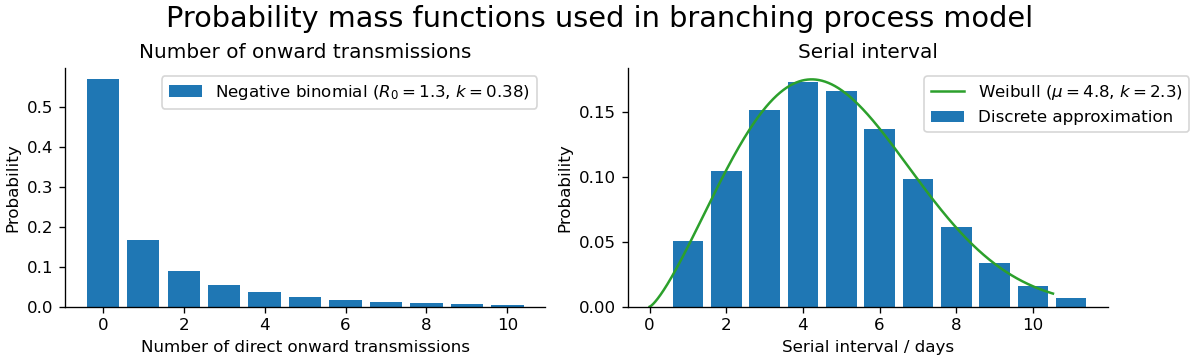
\includegraphics[width=\textwidth]{taiwan-model-distributions.png}
    \caption{The left plot shows the Negative Binomial distribution used to determine the number of onward infections, \(O_i\) directly caused by each individual \(i\). The right plot shows the distribution for the serial interval in days, with the continuous Weibull distribution used to generate it on top.}
    \label{fig:model-distributions}
\end{figure}

\autoref{fig:eoo-probabilities} shows the probability of future infections each day, assuming the branching process model and given the observations available up to and including that day.
Also shown in \autoref{fig:eoo-probabilities} is the following approximation to the probability which is used in \cite{Akhmetzhanov2021}, \cite{Linton2021} and \cite{Nishiura2016} (see \Cref{thm:approx-alternative} for latter equality)
\begin{equation}\label{eq:approximation}
\mathbb{P}(M(s) = 0 \;\forall s > t \;|\; \mathcal{D}) \approx \prod_{i=1}^n \sum_{f=0}^\infty \mathbb{P}(O = f) \mathbb{P}(S \leq t-t_i)^f = \prod_{i=1}^n \left(1 + \frac{pq_i}{1-p}\right)^{-k}
\end{equation}
where \(O\) has the same distribution as each of the direct transmission counts \(O_i\) and \(S\) has the same distribution as each of the serial intervals \(S_{ij}\).
We can see that the approximation is indeed mostly an over-estimate of the true probability as predicted in \cite{Nishiura2016}. However, comparing \autoref{eq:approximation} and \autoref{eq:conditional-eoo-prob} it isn't clear that it will always be an over-estimate, and indeed empirically we can see a small period at the beginning of the outbreak where the approximation is an under-estimate.
\autoref{fig:mcmc-example-trace} shows the trace of the Markov chain, using the date of the last infection as an example. From this we conclude that the chain is sufficiently mixed to trust the estimate for the end-of-outbreak probability obtained.

If the outbreak is declared over when the probability of future infections drops to 5\% or lower, then with the exact probability estimates calculated using MCMC, the outbreak would be declared over after 16th February, seven days after the last infection. Conversely, using the approximation the outbreak would be declared over after 18th February, nine days after the last infection.

\begin{figure}[p]
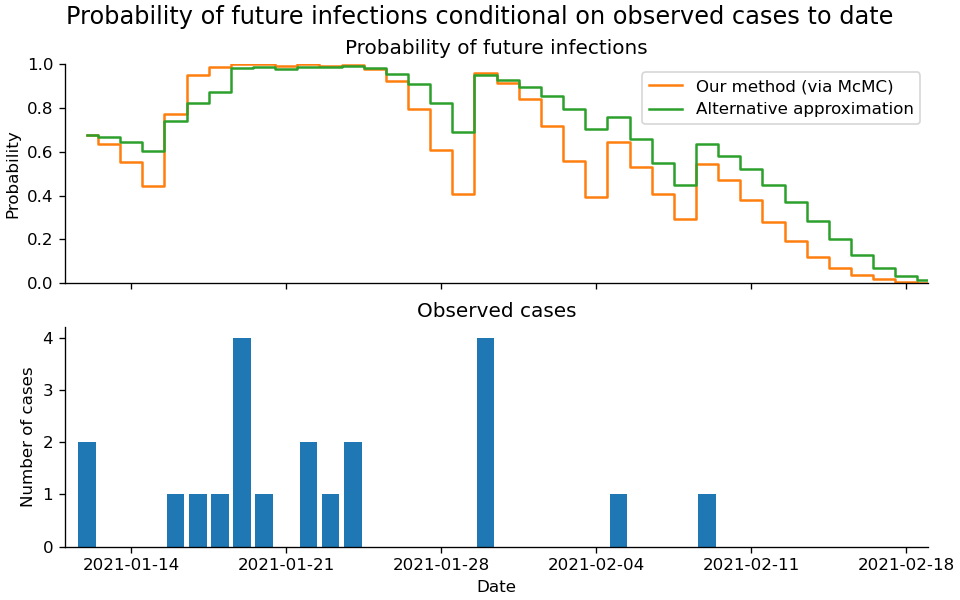
\includegraphics[width=\textwidth]{taiwan-eoo-plot.png}
\centering
\caption{Observed case counts from the outbreak by day (bottom) and the corresponding probability of future infection which would have been estimated at the end of each day (top) with both the MCMC estimate (orange) and the approximation (green). As expected in \cite{Nishiura2016}, the approximation mostly overestimates the probability of future infections, giving a more conservative threshold for declaring the outbreak over. If the outbreak is declared over when the probability of future infections drops below 5\% then with the exact method it would be declared over at the end of the day on 16th February, 7 days after the last observed case, while under the approximation it would be declared over at the end of the day on 18th February, 9 days after the last observed case.}
\label{fig:eoo-probabilities}
\end{figure}

\begin{figure}[p]
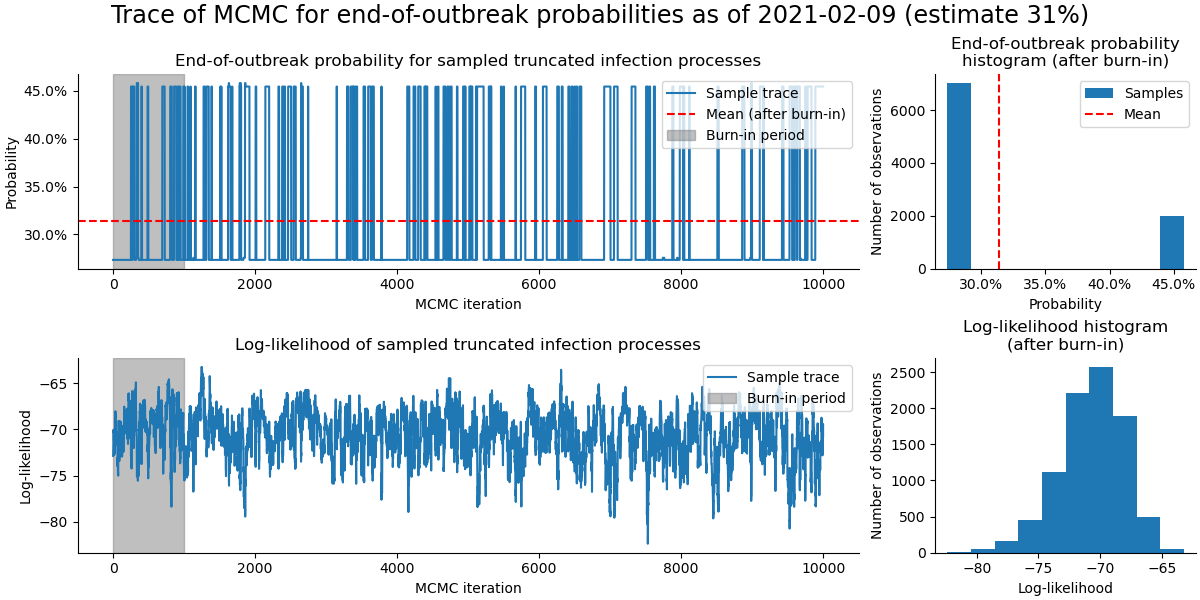
\includegraphics[width=\textwidth]{trace_28.png}
\centering
\caption{Trace for the Markov chain on the day of the last observed infection. The lower plots showing the log-likelihood of the infection graph show that the chain is well mixed for this purpose. The upper plots however, show that there are only two values taken by the end-of-outbreak probability. Most modifications to the infection graph do not affect the later infections and hence do not affect the end-of-outbreak probability and the resulting process is quite sticky. Consequently, while the estimate for the end-of-outbreak probability is still good, the effective sample size will be much smaller.}
\label{fig:mcmc-example-trace}
\end{figure}

\section{Conclusions}
I have shown that it is possible to use Markov Chain Monte Carlo to estimate the exact probability of future infections conditional on a set of observed cases, assuming that the imported infections are labelled. Further, the probabilities of future infections differ using the exact calculation compared with the approximation in \cite{Akhmetzhanov2021}, \cite{Linton2021} and \cite{Nishiura2016}, and the date that the outbreak is declared over at a 5\% risk threshold is brought forward by two days (22\%) in the example studied. However, I did not account for uncertainties in the model parameters, under-ascertainment of cases or reporting delay, which may all have a bigger effect on the end-of-outbreak date than the approximation.

%%  Future work cut out to improve page count:
% Possible further work to be done on this study includes:
% \begin{itemize}
%     \item Generating convergence statistics for the MCMC, as in \cite{Newman1999} to make it easier to assess convergence of the estimate for all dates;
%     \item Use distributions instead of point estimates for the parameters to give a credible interval for the end-of-outbreak probability, as in \cite{Akhmetzhanov2021} and \cite{Linton2021};
%     \item Account for the reporting delay as in \cite{Akhmetzhanov2021} and \cite{Linton2021};
%     \item Extend the method to account for under-ascertainment as in \cite{Linton2021} (using a different dataset where contact tracing was not conducted);
%     \item Run using online estimates of the parameters - the parameters used in this report were taken from \cite{Akhmetzhanov2021} where the full dataset was available to estimate the parameters.
% \end{itemize}

\FloatBarrier
\printbibliography

\appendix

\section{Appendix: Markov Chain Monte Carlo}\label{app:mcmc}
\textit{This section is heavily based on \cite{grimmett2020probability}.}

Markov Chain Monte Carlo is a method for sampling from a probability distribution \(\pi\) when we do not have access to the inverse of the cumulative distribution function. For example, we can estimate a sum of the form
\begin{equation}\label{eq:mcmc-expectation}
    \sum_{\theta \in \Theta} g(\theta) \pi(\theta)
\end{equation}
where \(g : \Theta \to \mathbb{R}\) and when we only know the probability mass function \(\pi\) on the sample space \(\Theta\) up to a multiplicative constant, say \(\pi = C \pi'\).

We sample from \(\pi\) by constructing an ergodic Markov chain \((X_n : n \geq 0)\) with stationary distribution \(\pi\). In the \(n\)th iteration of the Metropolis-Hastings algorithm, we choose the next value of the chain \(X_{n+1}\) with the following two step process:
\begin{enumerate}
    \item Propose a next value \(Y\) according to a proposal distribution \(h_{ij} = \mathbb{P}(Y=j | X_n=i)\).
    \item Accept the proposal with probability \(a_{ij}\) where
        \[a_{ij} = \min\left(1, \frac{\pi_j h_{ji}}{\pi_i h_{ij}}\right) = \min\left(1, \frac{\pi'_j h_{ji}}{\pi'_i h_{ij}}\right) \quad \forall i, j \in \Theta.\]
        If the proposal is accepted then set \(X_{n+1} = Y\), otherwise set \(X_{n+1} = X_n\).
\end{enumerate}
The choice of acceptance probability here ensures that the transition probabilities \(p_{ij} = h_{ij} a_{ij}\) satisfy the detailed balance equations and so the chain is reversible with respect to \(\pi\) and hence is ergodic.

\pagebreak[4]
\section{Appendix: Proofs of results on the branching process epidemic model}\label{app:proofs}
\textit{This section is entirely my own original work.}

\begin{lemma}\label{thm:nbinom-lemma}
Let \(O \sim \mathcal{NB}(k, p)\) be a negative binomial random variable, and let \(e \in \{0, 1, 2, \dots\}\) be a non-negative integer. Let \(q \in [0,1]\).
Then
\[\sum_{f=e}^\infty \mathbb{P}(O = f) \binom{f}{e} q^{f-e} = \underbrace{\frac{\Gamma(e+k)}{e! \Gamma(k)} p^e (1-p)^k}_{\mathbb{P}(O = e)} \frac{1}{(1-pq)^{e+k}}.\]
\end{lemma}

\begin{proof}
The mass function for the negative binomial variable, \(O\), is
\[
\forall f \in \{0, 1, \dots\}, \quad \mathbb{P}(O = f)
= \frac{\Gamma(f+k)}{f! \Gamma(k)} p^f (1-p)^k.
\]
Therefore
\begin{equation}\label{eq:app-lemma-eq1}
\sum_{f=e}^\infty \mathbb{P}(O = f) \binom{f}{e} q^{f-e}
= \frac{1}{e!}p^e (1-p)^k \sum_{f=e}^\infty \frac{\Gamma(f+k)}{(f-e)! \Gamma(k)} (pq)^{f-e}.
\end{equation}
If we differentiate the Taylor expansion for \(\frac{1}{(1-x)^k}\) with respect to \(x\) we obtain a series of the form on the right of \autoref{eq:app-lemma-eq1}
\begin{gather*}
    \frac{1}{(1-x)^k} = 1 + kx + \frac{1}{2!} k(k+1) x^2 + \frac{1}{3!} k(k+1)(k+2) x^3 + \dots = \sum_{f=0}^\infty \frac{\Gamma(f+k)}{f! \Gamma(k)} x^f \\
    \Rightarrow\quad \frac{d^e}{dx^e} \frac{1}{(1-x)^k} = \sum_{f=e}^\infty \frac{\Gamma(f+k)}{(f-e)!\Gamma(k)} x^{f-e}. \\
\end{gather*}
Differentiating this function in its original form gives a closed form expression for the infinite series
\begin{gather*}
    \frac{d^e}{dx^e} \frac{1}{(1-x)^k} = k(k+1)\dots(k+e-1) \frac{1}{(1-x)^{e+k}} = \frac{\Gamma(e+k)}{\Gamma(k)} \frac{1}{(1-x)^{e+k}} \\
    \Rightarrow\quad \sum_{f=e}^\infty \frac{\Gamma(f+k)}{(f-e)!\Gamma(k)} x^{f-e} = \frac{\Gamma(e+k)}{\Gamma(k)} \frac{1}{(1-x)^{e+k}}.
\end{gather*}
Substituting this into \autoref{eq:app-lemma-eq1} with \(x=pq\) gives
\[
\sum_{f=e}^\infty \mathbb{P}(O = f) \binom{f}{e} q^{f-e}
= \underbrace{\frac{\Gamma(e+k)}{e! \Gamma(k)} p^e (1-p)^k}_{\mathbb{P}(O = e)} \frac{1}{(1-pq)^{e+k}}
\]
completing the proof.

\end{proof}

\begin{proposition}\label{thm:conditional-eoo-prob}
Conditional on a particular infection graph, \(G_t\), explaining the infections observed up to time \(t\), the probability that there will be no future infections is
\[\mathbb{P}(M(s) = 0 \;\forall s > t \;|\; G_t, \mathcal{D}) = \prod_{i=1}^n (1-p q_i)^{e_i + k}\]
where \(p\), \(k\), \(\{q_i\}\), \(\{e_i\}\), \(M\) and \(\mathcal{D}\) are defined in \autoref{sec:background} and \autoref{sec:method}.
\end{proposition}

\begin{proof}
The probability that there will be no infections after time \(t\) is exactly the probability that \(O_i = e_i\) for all \(i\). Thus
\begin{align*}
\mathbb{P}(M(s) = 0 \;\forall s > t \;|\; G_t, \mathcal{D})
&= \mathbb{P}(O_i = e_i \;\forall i=1,\dots,n \;|\; G_t, \mathcal{D}) \\
&= \frac{\mathbb{P}(O_i = e_i \;\forall i=1,\dots,n ; G_t, \mathcal{D})}{\mathbb{P}(G_t, \mathcal{D})} \\
&= \frac{
    \prod_{i=1}^n \mathbb{P}(O_i = e_i) \overbrace{\prod_{j \in G_t :\, i \to j} \mathbb{P}(S_{ij} = s_{ij})}^{\text{cancels}}
}{
    \prod_{i=1}^n \sum_{f=e_i}^\infty \mathbb{P}(O_i = f) \binom{f}{e_i} \underbrace{\mathbb{P}(S > t-t_i)^{f-e_i}}_{q_i^{f-e_i}} \underbrace{\prod_{j \in G_t :\, i \to j} \mathbb{P}(S = s_{ij})}_{\text{cancels}}
} \\
&= \prod_{i=1}^n \frac{
    \mathbb{P}(O_i = e_i)
}{
    \sum_{f=e_i}^\infty \mathbb{P}(O_i = f) \binom{f}{e_i} q_i^{f-e_i}
} \\
&= \prod_{i=1}^n \frac{\mathbb{P}(O_i = e_i)}{\mathbb{P}(O_i = e_i) (1-pq_i)^{-(e_i+k)}} \qquad\text{by \Cref{thm:nbinom-lemma}} \\
&= \prod_{i=1}^n (1 - pq_i)^{e_i + k}.
\end{align*}
This completes the proof.
\end{proof}

\begin{proposition}\label{thm:conditional-graph-prob}
The probability of a particular infection graph \(G_t\) conditional on the observed case counts up to time \(t\) satisfies the following proportionality
\[
\mathbb{P}(G_t | \mathcal{D}) \propto 
\mathbb{P}(\mathcal{E} | \mathcal{D}) \prod_{i=1}^n \frac{1}{(1-pq_i)^{e_i + k}} \underbrace{\frac{\Gamma(e_i + k)}{e_i! \Gamma(k)} p^{e_i} (1-p)^k}_{\mathcal{NB}(k, p) \;\text{p.m.f.}} \prod_{j:\, i \to j} \mathbb{P}(S = s_{ij})
\]
where all notation is as defined in \autoref{sec:background} and \autoref{sec:method}.
\end{proposition}

\begin{proof}
As in \autoref{sec:background}, write \(\tilde{G}_t\) for the full branching process to time \(t\) generated by the infection graph \(G_t\) and observed infection times \(\mathcal{D}\). Then, noting that \(\tilde{G}_t\) entirely determines the imported infections \(\mathcal{E}\), we have
\begin{equation}\label{eq:graph-post-prop}
    \mathbb{P}(G_t | \mathcal{D})
    = \mathbb{P}(\tilde{G}_t | \mathcal{D})
    = \mathbb{P}(\tilde{G}_t, \mathcal{E} | \mathcal{D})
    = \mathbb{P}(\tilde{G}_t | \mathcal{D}, \mathcal{E}) \mathbb{P}(\mathcal{E} | \mathcal{D})
    \propto \underbrace{\mathbb{P}(\mathcal{D} | \tilde{G}_t, \mathcal{E})}_{=\mathbb{P}(\mathcal{D} | \tilde{G}_t)=1} \mathbb{P}(\tilde{G}_t | \mathcal{E}) \mathbb{P}(\mathcal{E} | \mathcal{D}).
\end{equation}
The first term here is just an indicator for whether the proposed branching process \(\tilde{G}_t\) would generate our observations \(\mathcal{D}\), which is always true by construction. The last term, \(\mathbb{P}(\mathcal{E} | \mathcal{D})\), is a distribution over which cases are imported cases, and is chosen by an expert. This leaves the middle term, which we can rewrite using \Cref{thm:nbinom-lemma}
\begin{align*}
    \mathbb{P}(\tilde{G}_t | \mathcal{E}) &= \prod_{i=1}^n \sum_{f=e_i}^\infty \mathbb{P}(O_i = f) \binom{f}{e_i} q_i^{f-e_i} \prod_{j:\, i \to j} \mathbb{P}(S_{ij} = s_{ij}) \\
    &= \prod_{i=1}^n \frac{1}{(1-pq_i)^{e_i + k}} \mathbb{P}(O_i = e_i) \prod_{j:\, i \to j} \mathbb{P}(S_{ij} = s_{ij}) \\
    &= \prod_{i=1}^n \frac{1}{(1-pq_i)^{e_i + k}} \underbrace{\frac{\Gamma(e_i + k)}{e_i! \Gamma(k)} p^{e_i} (1-p)^k}_{\mathcal{NB}(k, p) \;\text{p.m.f.}} \prod_{j:\, i \to j} \mathbb{P}(S = s_{ij}).
\end{align*}
Substituting this into \autoref{eq:graph-post-prop} completes the proof.

\end{proof}

\begin{proposition}\label{thm:approx-alternative}
The end-of-outbreak approximation from \cite{Akhmetzhanov2021}, \cite{Linton2021} and \cite{Nishiura2016} can be rewritten as
\[\prod_{i=1}^n \sum_{f=0}^\infty \mathbb{P}(O = f) \mathbb{P}(S \leq t-t_i)^f = \prod_{i=1}^n \left(1 + \frac{pq_i}{1-p}\right)^{-k}.\]
\end{proposition}

\begin{proof}
We will show that the \(i\)th term in the product is the same for each expression. Let \(i \in \{1, \dots, n\}\). Then
\begin{align*}
    \sum_{f=0}^\infty \mathbb{P}(O = f) \mathbb{P}(S \leq t-t_i)^f
    &= \sum_{f=0}^\infty \frac{\Gamma(f+k)}{f! \Gamma(k)} p^f (1-p)^k (1-q_i)^f \\
    &= \frac{(1-p)^k}{(1-p(1-q_i))^k} \sum_{f=0}^\infty \underbrace{\frac{\Gamma(f+k)}{f! \Gamma(k)} (p(1-q_i))^f  (1-p(1-q_i))^k}_{\mathcal{NB}(k, p(1-q_i)) \;\text{p.m.f.}} \\
    &= \left(\frac{1-p}{1-p+pq_i}\right)^k \\
    &= \left(1 + \frac{pq_i}{1-p}\right)^{-k}.
\end{align*}

\end{proof}

\end{document}
